
\section{A \texorpdfstring{$\varphi$--$\pi$--$\e$}{phi--pi--e} template for the Standard Model interface}
\label{sec:sm_interface}

This section records the physical identification layer: falsifiable mapping hypotheses that connect the three-channel folding template to Standard Model structures.

\subsection{Three channels as three compensation classes}
\label{subsec:gauge_as_compensation}

The folding framework isolates three commuting stability channels:
\begin{itemize}
\item \textbf{($\varphi$) syntactic legality.} A forbidden-word grammar (Zeckendorf admissibility).
\item \textbf{($\pi$) topological closure.} A cyclic monodromy / wrap-around admissibility condition.
\item \textbf{($\e$) analytic stability.} A zeta/Abel holomorphy domain with a pole barrier.
\end{itemize}

Independently, the Standard Model gauge group is a three-factor product $SU(3)\times SU(2)\times U(1)$ \cite{PeskinSchroeder1995}.
We first record the protocol-level necessity of compensation under cross-site consistency, and then record a CAP-minimal gauge-factor closure under explicit compactness and factorization constraints that are forced by probability-preserving internal redundancy (Proposition~\ref{prop:unitary_implies_compact_redundancy}) and by channelwise independence (Lemma~\ref{lem:three_channel_factorization}).

\begin{proposition}[Finite-fiber mismatch forces a compensating connection datum (interface)]
\label{prop:gauge_compensation}
Fix a window length $m$ and an addressing graph that renders a finite tick prefix as a locality structure (Section~\ref{sec:tick_calculus}; e.g.\ the Hilbert-addressed grid at order $n=3$).
Let each site $x$ carry a stable label $w_x\in X_m$ and let its microstate fiber be
\[
P(w_x):=\mathrm{Fold}_m^{-1}(w_x)\subset\{0,\dots,2^m-1\},
\]
so that multiple microscopic indices can project to the same stable readout label.
If protocol-consistent comparison/transport of stable labels is required across a neighbor edge $x\sim y$, then the stable labels alone are insufficient: one must specify an additional transport rule that matches the endpoint fibers.
After embedding endpoint fibers into a common slot set of size $r:=\max_{w\in X_m}|P(w)|$ (by any deterministic padding convention), any such edge transport is represented by a permutation in $S_r$.
Changing the local slot labeling at a vertex acts by conjugation on edge transports, so the transport rule is defined only up to local relabelings (a finite gauge redundancy).
In a continuum modeling dictionary, such discrete connection data are represented by gauge connections on a bundle.
\end{proposition}
\begin{proof}
The point is finite and protocol-internal.
When $|P(w)|>1$, the stable label $w$ identifies only an equivalence class of microstates, so comparing two neighboring stable labels requires a choice of how the two equivalence classes are matched.
Once a uniform slot count $r$ is fixed, such matchings are elements of the finite symmetry group $S_r$.
Local relabelings at vertices change edge matchings by left/right multiplication and therefore conjugate loop products, which is the standard discrete gauge-transformation law on graphs \cite{Wilson1974,Rothe2012}.
At the minimal anchor $m=6$ one has $r=4$, and Section~\ref{sec:protocol_connections_holonomy} gives an explicit deterministic construction of an $S_4$ edge connection and its plaquette holonomy diagnostics.
\end{proof}

\paragraph{Assumption bundle for gauge-factor closure (audit).}
\AuditTag For audit clarity, Proposition~\ref{prop:channel_to_gauge} should be read as a conditional interface closure under an explicit assumption bundle:
\begin{itemize}
\item \textbf{(G1) Channelwise factorization.} The three commuting defect channels correspond to three independent local redundancy sectors (Lemma~\ref{lem:three_channel_factorization}).
\item \textbf{(G2) Compact probability-preserving redundancy.} In a continuum dictionary, internal redundancy is represented by probability-preserving transformations on a finite-dimensional local Hilbert space, hence is compact at the connected level (Proposition~\ref{prop:unitary_implies_compact_redundancy}).
\item \textbf{(G3) Candidate family.} The non-abelian redundancy closes to two simple compact factors $G_2,G_3$ (non-isomorphic) together with the $U(1)$ sector forced by local rephasing (Proposition~\ref{prop:local_rephasing_connection}).
In the present paper, the candidate-family component is supplied by the following protocol-internal interface route:
\textbf{(G3c) holonomy-diagnostic route} (Definition~\ref{def:holonomy_to_candidate_family_rule} in Appendix~\ref{app:gauge3_holonomy_candidate_closure}).
For readers who prefer alternative underwritings, we also record two optional corroboration routes:
\textbf{(G3a) physics-consensus route} (Assumption~\ref{ass:consensus_three_factor_gauge} in Appendix~\ref{app:physics_consensus_inputs})
and \textbf{(G3b) optional microscopic Q route} (Assumption~\ref{ass:m2star_internal_fiber_g2}; Lemma~\ref{lem:three_channel_8_state_minimal_record}; Proposition~\ref{prop:hurwitz_normed_division_algebras}; Proposition~\ref{prop:qcomp_implies_qwave_weak}; Corollary~\ref{cor:octonion_three_channel_minimality} in Appendix~\ref{app:internal_fiber_g2_optional}; together with Lemma~\ref{lem:z128_interference_vs_mixture} in Appendix~\ref{app:quantum_measurement_born}).
No equivalence between these routes is assumed.
\item \textbf{(G4) Complexity label and tie-break.} CAP selects the lexicographically minimal factor pair under a declared discrete complexity label; the main text uses $\dim(\mathfrak{g})$, and Appendix~\ref{app:gauge_complexity_sensitivity} audits sensitivity to alternative labels.
\end{itemize}

\begin{proposition}[CAP-minimal three-factor gauge closure (interface)]\label{prop:channel_to_gauge}
Fix a continuum modeling dictionary in which the compensation redundancy is internal and probability-preserving (hence compact at the connected level; Proposition~\ref{prop:unitary_implies_compact_redundancy}) and in which the three defect channels define three independent redundancy sectors (Lemma~\ref{lem:three_channel_factorization}).
Equip compact gauge factors with the intrinsic complexity label $\dim(\mathfrak{g})$ (Lie-algebra dimension) and select the lexicographically minimal triple, under CAP (Axiom~\ref{ax:cap}), among compact gauge groups of the form
\[
U(1)\times G_2\times G_3,
\]
where $G_2$ and $G_3$ are compact, non-abelian, simple, and non-isomorphic.
Then the unique minimizer is $U(1)\times SU(2)\times SU(3)$ (up to finite group quotients).
\end{proposition}
\begin{proof}
By Proposition~\ref{prop:local_rephasing_connection}, local rephasing redundancy enforces an abelian $U(1)$ connection sector in any local continuum dictionary.
Compact Lie algebras split as a direct sum of an abelian torus algebra and compact simple factors; requiring two additional inequivalent non-abelian simple factors and applying minimality in $\dim(\mathfrak{g})$ selects dimensions $3$ and $8$, hence $\mathfrak{su}(2)$ and $\mathfrak{su}(3)$ by Lemma~\ref{lem:su2_su3_unique_by_dim}.
\end{proof}

The content of Proposition~\ref{prop:gauge_compensation} is operational: gauge redundancy arises because compensation is only defined up to local rephasing of the readout basis.
The three-factor structure is not assumed as a premise, but closed as a CAP-minimal identification within the stated compactness/factorization constraints (Proposition~\ref{prop:channel_to_gauge}).

\begin{proposition}[Three commuting defect channels force a three-factor compensation structure (interface)]\label{prop:three_factor_compensation}
Suppose protocol mismatch certificates decompose into three commuting defect channels and that, at the modeling level, compensation is defined only up to independent local basis changes associated with each channel (the channelwise redundancy stance of Lemma~\ref{lem:three_channel_factorization}).
Then the minimal compensating connection splits into three independent connection components, so the effective local redundancy factorizes into a product of three gauge redundancies.
\end{proposition}
\begin{proof}
Since the defect channels commute, a mismatch certificate can be represented as a triple of channelwise components and compared channel-by-channel.
By the channelwise redundancy stance, each channel admits its own local basis redundancy, so at each site $x$ the modeling dictionary permits independent local changes $(g_\varphi(x),g_\pi(x),g_\e(x))$.
Consequently, any channelwise covariant transport rule along an edge $x\sim y$ is a triple of group elements
\[
(A_\varphi,A_\pi,A_\e)_{x\to y}\in G_\varphi\times G_\pi\times G_\e,
\]
transforming under local basis changes as
\[
(A_\varphi,A_\pi,A_\e)_{x\to y}\ \mapsto\
\bigl(g_\varphi(y)A_\varphi g_\varphi(x)^{-1},\ g_\pi(y)A_\pi g_\pi(x)^{-1},\ g_\e(y)A_\e g_\e(x)^{-1}\bigr).
\]
Thus the minimal redundancy group is the direct product of the three independent channel redundancies.
\end{proof}

\paragraph{Uniqueness at the Lie-algebra level.}
Under probability-preserving internal redundancy (hence compactness at the connected level; Proposition~\ref{prop:unitary_implies_compact_redundancy}) and using Lie-algebra dimension as an intrinsic complexity label, the dimensions $(1,3,8)$ already pin the factor Lie algebras uniquely to $\mathfrak{u}(1)\oplus\mathfrak{su}(2)\oplus\mathfrak{su}(3)$ (up to finite group quotients), by the Cartan--Killing classification (Lemma~\ref{lem:su2_su3_unique_by_dim}).
In this sense, once the three-channel template is fixed and one commits to dimension-as-complexity, the choice of $U(1)$, $SU(2)$, and $SU(3)$ is rigid rather than a naming convention.
Appendix~\ref{app:gauge_complexity_sensitivity} records a bounded sensitivity sweep showing that the same minimizer persists under several alternative discrete complexity labels in the tested window.
Moreover, Proposition~\ref{prop:gauge_label_robustness} gives a short theorem-level reason for this robustness for the most natural low-complexity labels (dimension, rank, dimension+rank, and $d_{\min}$).

\paragraph{Compensation as a locality cost.}
In the finite protocol language, a gauge field is not an extra substance but the bookkeeping of enforcing phase consistency across neighboring addresses.
When the local stable sector is defined by defect suppression, neighboring sites generically disagree on which microstates project to which stable types.
A compensating connection is the minimal additional datum required to compare (and transport) stable types between sites without ambiguity.
In this paper, we formulate this as an implementation budget: compensation has a cost, and the effective dynamics favors minimal discrepancy subject to protocol constraints (Axiom~\ref{ax:cap}).

\paragraph{Rigidity and defects.}
In topologically trivial regions a compensating connection can be gauged away (pure gauge), while persistent mismatch requires nontrivial holonomy supported by defects.
This aligns the ``matter as defect'' view with the ``gauge as compensation'' view: matter is a stable obstruction that prevents global trivialization of the connection.

\begin{proposition}[From local rephasing to a connection field (standard)]\label{prop:local_rephasing_connection}
Let $\psi(x)$ be a complex matter field and impose local $U(1)$ redundancy $\psi(x)\mapsto \e^{\iu\lambda(x)}\psi(x)$.
Then invariance of a local kinetic term under this redundancy requires introducing a compensating connection $A_\mu$ and replacing $\partial_\mu$ by the covariant derivative $D_\mu=\partial_\mu-\iu A_\mu$.
Assuming locality and Lorentz covariance and restricting to bulk terms quadratic in $A_\mu$ and its first derivatives, the unique gauge-invariant quadratic kinetic term is proportional to $F_{\mu\nu}F^{\mu\nu}$, where $F_{\mu\nu}=\partial_\mu A_\nu-\partial_\nu A_\mu$.
\end{proposition}
\begin{proof}
This is standard; see, e.g., \cite{Weyl1929,PeskinSchroeder1995,WeinbergQFT1995}.
\end{proof}

\begin{proposition}[From local \texorpdfstring{$SU(N)$}{SU(N)} redundancy to a Yang--Mills connection (standard)]\label{prop:local_sun_connection}
Let $\psi(x)$ transform in a representation of $SU(N)$ and impose local redundancy $\psi(x)\mapsto U(x)\psi(x)$ with $U(x)\in SU(N)$.
Then invariance of a local kinetic term under this redundancy requires introducing an $SU(N)$ connection $A_\mu(x)$ and replacing $\partial_\mu$ by the covariant derivative $D_\mu=\partial_\mu-\iu g\,A_\mu$.
The corresponding curvature (field strength) is
\[
F_{\mu\nu}:=\frac{\iu}{g}[D_\mu,D_\nu]=\partial_\mu A_\nu-\partial_\nu A_\mu-\iu g\,[A_\mu,A_\nu],
\]
and, restricting to local bulk terms quadratic in $F_{\mu\nu}$, the gauge-invariant kinetic term is proportional to $\Tr(F_{\mu\nu}F^{\mu\nu})$.
\end{proposition}
\begin{proof}
Standard; see, e.g., \cite{YangMills1954,PeskinSchroeder1995,WeinbergQFT1995}.
\end{proof}

\begin{remark}[Relation to the CAP gauge-field viewpoint]\label{rem:cap_gauge_fields_pointer}
The standard continuum statements above are included only as a matching dictionary: they translate local basis redundancy into the familiar connection-field language.
In the HPA--$\Omega$ program, the same structural conclusion---that a compensating connection is forced once local phase consistency is demanded---is developed directly from finite readout and CAP-minimal discrepancy logic; see the companion CAP manuscript \cite{Ma2025CAP} for an extended presentation.
\end{remark}

\subsection{Stable types as minimal defect-carrying modes}
\label{subsec:matter_as_types}

In the protocol viewpoint adopted here, matter is modeled as persistent topological defects whose stability is constrained by an implementation budget.
In the present finite-resolution setting, the stable types $X_6$ provide a minimal, explicitly enumerable set of defect labels.

\begin{definition}[Particles as stable types (interface)]
\label{def:particles_as_types}
Physical particle labels at the chosen anchor scale are identified with stable readout types in $X_6$ (or with protocol-invariant functionals thereof), while microstates in $\Omega_6\setminus X_6$ are protocol-unstable and do not survive as visible outputs under projection.
\end{definition}

\paragraph{Micro/macro unification pointer (contract form).}
\AuditTag The particle-as-type identification above is complemented by a unified dynamical contract used later:
micro stabilization overhead is read as scattering delay (mass-as-latency), trapping is treated as a horizon-like surrogate only within declared protocols,
and any wormhole-like shortcut is a paid pointer-jump channel subject to the full-fusion hard gates.
See Section~\ref{subsec:micro_bh_wh_particle_unification}, Section~\ref{subsec:x3a_wormhole_rigidity_unified_constraints}, and
Proposition~\ref{prop:four_way_unification_contract_form}.

The $18\oplus 3$ split of $X_6$ then becomes a structural interface candidate:
boundary types are non-closed readout defects (endpoints), while cyclic types are closed defects (loops).
This matches the qualitative distinction between colorless endpoint-like excitations and loop-carrying excitations that can support nontrivial holonomy.

\begin{table}[t]
\centering
\small
\setlength{\tabcolsep}{10pt}
\renewcommand{\arraystretch}{1.15}
\begin{tabular}{lll}
\toprule
protocol object & count & Standard Model interface target \\
\midrule
cyclic stable types $X_6^{\mathrm{cyc}}$ & $18$ & $3$ generations $\times$ $(Q_L,u_R,d_R,L_L,e_R,\nu_R)$ \\
boundary stable types $X_6^{\mathrm{bdry}}$ & $3$ & gauge-factor connection classes $\{U(1),SU(2),SU(3)\}$ \\
\bottomrule
\end{tabular}
\caption{A compact $18\oplus 3$ interface map at the anchor: cyclic stable types are mapped to chiral fermion multiplets (with the minimal anomaly-neutral $\nu_R$ extension), while boundary stable types are mapped to the three gauge-factor connection classes. The full explicit labeling table is recorded in Table~\ref{tab:sm_labeling_table}.}
\label{tab:hpa_18_3_sm_interface}
\end{table}

\paragraph{Why the \texorpdfstring{$18\oplus 3$}{18+3} split is a rigid interface constraint.}
The split is enforced by a concrete wrap-around defect predicate $D_\pi$, hence has an intrinsic ``closure vs endpoint'' meaning at the protocol level.
Interpreting cyclic types as loop-like carriers and boundary types as endpoint-like carriers is therefore not an analogy but a direct reading of the $\pi$-constraint.
The numbers also provide a rigid counting target: any SM identification must explain why exactly $18$ stable types admit closure while exactly $3$ do not at the anchor scale.

\paragraph{A rigid integer pattern tying 21 to SM data.}
Beyond closure semantics, the minimal stable count admits a nontrivial arithmetic decomposition that matches Standard Model integers used elsewhere in this paper:
\[
|X_6|=21=(18+3)=(8+3)+10.
\]
Here $8=\dim(\mathfrak{su}(3))$ and $3=\dim(\mathfrak{su}(2))$ are the gauge-sector dimensions, while $10=\sum_{f\in\mathrm{SM}}Y_f^2$ is the hypercharge-squared sum over the chiral fermion content in three generations under the PDG normalization $Q=T_3+Y$.
The identity $21=(8+3)+10$ is an integer constraint and does not involve any post-hoc fitting freedom; it is recorded as an auditable counting target for the closed labeling interface (Proposition~\ref{prop:sm_labeling_closed}).
The same integers reappear in the electroweak normalization ($13=10+3$; Section~\ref{subsec:weinberg_angle}) and in the CP-odd multiplicity ($d_{\mathrm{CP}}=8+3$; Section~\ref{subsec:cp_jarlskog}), providing a cross-checked integer backbone across multiple independent interface diagnostics.

\begin{lemma}[Hypercharge-squared sum $\sum Y^2$]\label{lem:hypercharge_sum_10}
Under the PDG convention $Q=T_3+Y$ \cite{PDGRPP2024}, the Standard Model chiral fermion content without right-handed neutrinos satisfies
\[
\sum Y^2=\frac{10}{3}\quad\text{per generation},
\qquad
\sum_{f\in\mathrm{SM}}Y_f^2=10\quad\text{for three generations}.
\]
\end{lemma}
\begin{proof}
For one generation, sum $Y^2$ over left-handed Weyl fields with multiplicities (color and weak components):
\[
6\left(\frac{1}{6}\right)^2
 +3\left(\frac{2}{3}\right)^2
 +3\left(\frac{1}{3}\right)^2
 +2\left(\frac{1}{2}\right)^2
 +1\cdot (1)^2
=\frac{10}{3},
\]
corresponding to $Q_L$, $u_R$, $d_R$, $L_L$, and $e_R$.
Multiplying by three generations yields $10$.
A sterile singlet $\nu_R$ has $Y=0$ and does not change the sum.
\end{proof}

\subsection{Minimal mapping problem}
\label{subsec:min_mapping_problem}

We record the interface as an explicit mapping problem.
A closed, computable field-level labeling map is provided in Section~\ref{sec:sm_labeling_closure}.
\paragraph{How the closed labeling is constructed (preview).}
The labeling closure is not an unstructured guess: it is a deterministic order-isomorphism between two finite totally ordered sets.
On the protocol side, the $18$ cyclic stable types are totally ordered by intrinsic invariants (Definition~\ref{def:r_star} and Definition~\ref{def:order_x6}).
On the Standard Model side, the $18$ chiral multiplets are totally ordered by the tuple $(g,\dim(SU(3)\text{-rep}),(6Y)^2,\dim(SU(2)\text{-rep}),\text{name})$ under the PDG convention $Q=T_3+Y$ (Definition~\ref{def:order_fsm}).
Matching ranks yields a unique cyclic assignment, while the three boundary types are assigned to $\{U(1),SU(2),SU(3)\}$ by monotone matching of intrinsic value and gauge-sector complexity (Lemma~\ref{lem:gauge_dim_order}); see Theorem~\ref{thm:labeling_unique} and Table~\ref{tab:sm_labeling_table}.

\begin{definition}[Intrinsic invariants available at window length $6$]\label{def:x6_invariants}
For $w\in X_6$, the finite protocol provides several intrinsic, directly computable invariants:
\begin{itemize}
\item \textbf{closure/boundary tag:} $D_\pi(w)\in\{0,1\}$ (cyclic vs.\ boundary);
\item \textbf{Zeckendorf value:} $V(w)\in\{0,\dots,20\}$ (Definition~\ref{def:zeckendorf_value});
\item \textbf{Hamming weight:} $|w|_1\in\{0,1,2,3\}$ (Appendix~\ref{app:generated_tables});
\item \textbf{folding degeneracy:} $g(w):=|\mathrm{Fold}_6^{-1}(w)|\in\{2,3,4\}$ (Theorem~\ref{thm:fold6_stats}).
\end{itemize}
\end{definition}

\begin{proposition}[Closed Standard Model labeling at $(m,n)=(6,3)$]\label{prop:sm_labeling_closed}
The Standard Model labeling of the $21$ stable types at the chosen anchor $(m,n)=(6,3)$ is closed and unique:
Theorem~\ref{thm:labeling_unique} constructs a unique split-compatible labeling map $\mathcal{L}_{\mathrm{SM}}:X_6\to \mathcal{F}_{\mathrm{SM}}\sqcup\mathcal{G}_{\mathrm{SM}}$ by order isomorphism on the cyclic sector and the unique monotone assignment on the boundary sector.
Moreover, under window uplift $m\mapsto m'$ the labeling admits a canonical functorial lift by prefix projection together with explicit refinement multiplicities and deterministic refinement indices (Appendix~\ref{app:functorial_refinement}).
\end{proposition}

\subsection{No-Go Theorem: the scalar exclusion principle (interface)}
\label{subsec:scalar_sectors_interface}

At the chosen anchor instance $(m,n)=(6,3)$, the $21$-type interface is optimized for a chiral/gauge closure:
$18$ cyclic labels for chiral fermion multiplets and $3$ boundary labels for gauge-factor classes (Section~\ref{sec:sm_labeling_closure}).
In this setting we record a no-go statement on the physical identification layer:
the scalar sector is \emph{not} realized by an additional primitive stable-type label at the minimal window.
\InterfaceTag The primary obstruction is combinatorial and audit-complete: under the closed $21$-type contract at the anchor, every stable type in $X_6$ is already consumed by the chiral/gauge labeling map, leaving no unused label for an additional Higgs-like primitive type (Proposition~\ref{prop:higgs_not_in_x6_forced}).
Accordingly, scalar behavior must enter either as (i) an EFT-level completion field in a continuum dictionary, or (ii) a protocol-emergent observable supported by resolution uplift and coarse graining (Proposition~\ref{prop:higgs_not_in_x6_forced} and Proposition~\ref{prop:scalar_sector_closed}).

\paragraph{The vector nature of the linear universe (interface).}
\AuditTag Under Axiom~\ref{ax:readout_sequentiality} the primitive ontology is a directed scan: the microscopic description is not a static configuration but an ordered stream.
At the minimal anchor, several intrinsic invariants used for chiral/gauge closure are explicitly tied to directional protocol data (scan order and the chirality sign datum in the Hilbert family).
From this viewpoint, parity-even scalar behavior is naturally modeled only after coarse graining and/or uplift, where directional data averages out (Remark~\ref{rem:scalar_emergent_route} and Appendix~\ref{app:scalar_interface_audits}).

\begin{remark}[Relation to composite/Goldstone Higgs paradigms]\label{rem:composite_higgs_relation}
Treating the Higgs doublet as an EFT-level degree of freedom rather than a primitive elementary mode is compatible with mature composite/Goldstone Higgs frameworks, in which a scalar arises as an emergent low-energy excitation of a more microscopic sector; see, e.g., \cite{Contino2011TASICompositeHiggs,PanicoWulzer2016CompositeHiggs}.
The present protocol formulation differs in microscopic language, but it implies the same practical expectation: scalar behavior can be resolution-dependent and should admit additional diagnostic constraints beyond a minimal chiral labeling at $m=6$.
\end{remark}

In particular, a renormalizable Standard Model EFT includes a scalar Higgs doublet whose vacuum structure controls electroweak symmetry breaking.
In the present protocol language, the Higgs is therefore treated as an EFT-level completion (Appendix~\ref{app:protocol_eft_embedding}) rather than as an additional minimal stable type at $m=6$ (Remark~\ref{rem:higgs_not_in_21}).
The resolution-uplift narrative fixes a concrete locus for scalar emergence:
in the admissible-set sweep one has $|X_{10}|=144=123\oplus 21$ (Table~\ref{tab:xm_sweep}), and under the minimal staircase calibration the threshold for $m=10$ lies near the electroweak scale (Section~\ref{subsec:p3_resolution_jumps}, Table~\ref{tab:resolution_thresholds}).
Accordingly, in the present interface language electroweak-scalar behavior is modeled as an emergent, parity-even background supported by higher-resolution texture, not as a primitive type at the minimal window.

\begin{proposition}[Scalar-sector closure in the protocol language]\label{prop:scalar_sector_closed}
At the minimal stable alphabet $(m,n)=(6,3)$, parity-even scalar modes are closed as protocol-emergent observables rather than as additional primitive stable types:
\begin{itemize}
\item \textbf{(parity-even scalar observables)} Coarse-grained scalar observables are obtained by spatial block-averaging intrinsic stable-type functionals on the Hilbert-addressed grid (Definition~\ref{def:coarse_grained_scalar}); by construction they are invariant under $P_{\mathrm{prot}}$ up to pullback (Remark~\ref{rem:scalar_emergent_route}).
\item \textbf{(coupling to compensating connections)} In a lattice-gauge modeling dictionary, scalar site variables couple to link connections by gauge-covariant nearest-neighbor terms that reduce to $(D_\mu H)^\dagger(D^\mu H)$ in a continuum limit \cite{Wilson1974,KogutSusskind1975HamiltonianLGT,Rothe2012}; in protocol language this corresponds to allowing the local implementation cost of transport/holonomy to depend on a coarse-grained scalar observable (Remark~\ref{rem:scalar_emergent_route} and Remark~\ref{rem:protocol_eft_status}).
\item \textbf{(uplift dependence)} A distinct scalar ``type'' is therefore expected only under resolution uplift and coarse graining, not as a new label in $X_6$; the first audited locus is the $m=10$ uplift where $|X_{10}|=144=123\oplus 21$ and the staircase calibration places $\mu_{\mathrm{th}}(10)$ near the electroweak scale (Table~\ref{tab:xm_sweep} and Table~\ref{tab:resolution_thresholds}).
\end{itemize}
\end{proposition}

\paragraph{Quantitative scalar-scale closure (supplement).}
\AuditTag The bounded-denominator Higgs--$Z$ depth-offset rigidity audit is recorded in Appendix~\ref{app:scalar_interface_audits} (Proposition~\ref{prop:higgs_z_offset_rigidity}, Table~\ref{tab:higgs_z_offset_sweep}).

\begin{definition}[Coarse-grained protocol scalars]\label{def:coarse_grained_scalar}
Fix a Hilbert order $n$ and view the scan index as embedded on the grid by $H_n$ (Section~\ref{sec:hilbert_addressing}).
Let $q$ be any intrinsic protocol functional on stable types (for example $q(w)\in\{V(w),|w|_1,g(w),D_\pi(w)\}$ at $m=6$).
A \emph{coarse-grained scalar observable} is any block-averaged field obtained by spatial averaging of $q$ over a finite neighborhood on the Hilbert-addressed grid.
Block averaging as a coarse-graining operation is standard in lattice models; see, e.g., \cite{Wilson1974,Rothe2012}.
\end{definition}

\begin{remark}[A minimal protocol route to scalar effective modes]\label{rem:scalar_emergent_route}
By construction, coarse-grained observables of Definition~\ref{def:coarse_grained_scalar} are parity-even in the protocol sense: under $P_{\mathrm{prot}}$ they transform by pullback of the spatial reflection on the grid rather than by an intrinsic sign flip.
They are likewise insensitive to the traversal-direction sign datum used to define the discrete chirality index $\chi$.
This provides a concrete protocol interpretation for a scalar exclusion at the minimal stable alphabet: parity-even scalar modes are naturally modeled as composite or protocol-emergent observables whose appearance depends on coarse graining and resolution uplift, consistent with the Higgs-sector status recorded in Remark~\ref{rem:higgs_not_in_21}.
\end{remark}

\paragraph{A minimal finite check (supplement).}
\AuditTag The parity-contrast check between the chirality sign datum and coarse-grained scalar summaries is recorded in Appendix~\ref{app:scalar_interface_audits} (Table~\ref{tab:scalar_coarse_grain}).

\paragraph{A canonical Higgs-like scalar doublet from uplift microtexture (interface).}
\InterfaceTag At the anchor $(m,n)=(6,3)$ the $21$ stable types are fully consumed by the $18\oplus 3$ chiral/gauge labeling contract, hence no additional primitive Higgs label exists (Proposition~\ref{prop:higgs_not_in_x6_forced}).
At the first audited uplift locus $m=10$ (Proposition~\ref{prop:scalar_sector_closed}), the protocol nonetheless carries additional microstructure beyond the $X_6$ label by functorial prefix projection.
Concretely, fix the balanced $2$D Hilbert screen at order $n=5$ and embed the first $2^{10}$ scan indices by the Hilbert map $H_5$.
For each occupied site $x$ with scan index $k$, let
\[
w(x):=\mathrm{Fold}_{10}(k)\in X_{10},
\qquad
u(x):=\pi_{10\to 6}(w(x))\in X_6.
\]
The $18\oplus 3$ particle/gauge label at $x$ is $\mathcal{L}_{\mathrm{SM}}(u(x))$, while the uplift microtexture is carried by the suffix bits of $w(x)$.
Define four protocol-local scalar channels
\[
b_j(x):=w_{6+j}(x)\in\{0,1\},
\qquad j\in\{0,1,2,3\},
\]
and their coarse-grained versions by $4\times 4$ block averaging on the Hilbert screen.
\InterfaceTag A canonical Higgs-doublet representative is obtained by bundling the four real scalar channels into two complex components,
\[
H_1:=\overline{b}_0+\iu\,\overline{b}_3,
\qquad
H_2:=\overline{b}_1+\iu\,\overline{b}_2,
\]
where $\overline{b}_j$ denotes the stated block average.
This construction is deterministic at fixed $(m,n)$ and provides an explicit protocol-level realization of a parity-even scalar doublet supported by uplift microtexture, consistent with the scalar-sector closure principle.
The corresponding audit artifacts and the $3$D Hilbert-screen instance are recorded in Appendix~\ref{app:scalar_interface_audits}.

\begin{figure}[t]
\centering
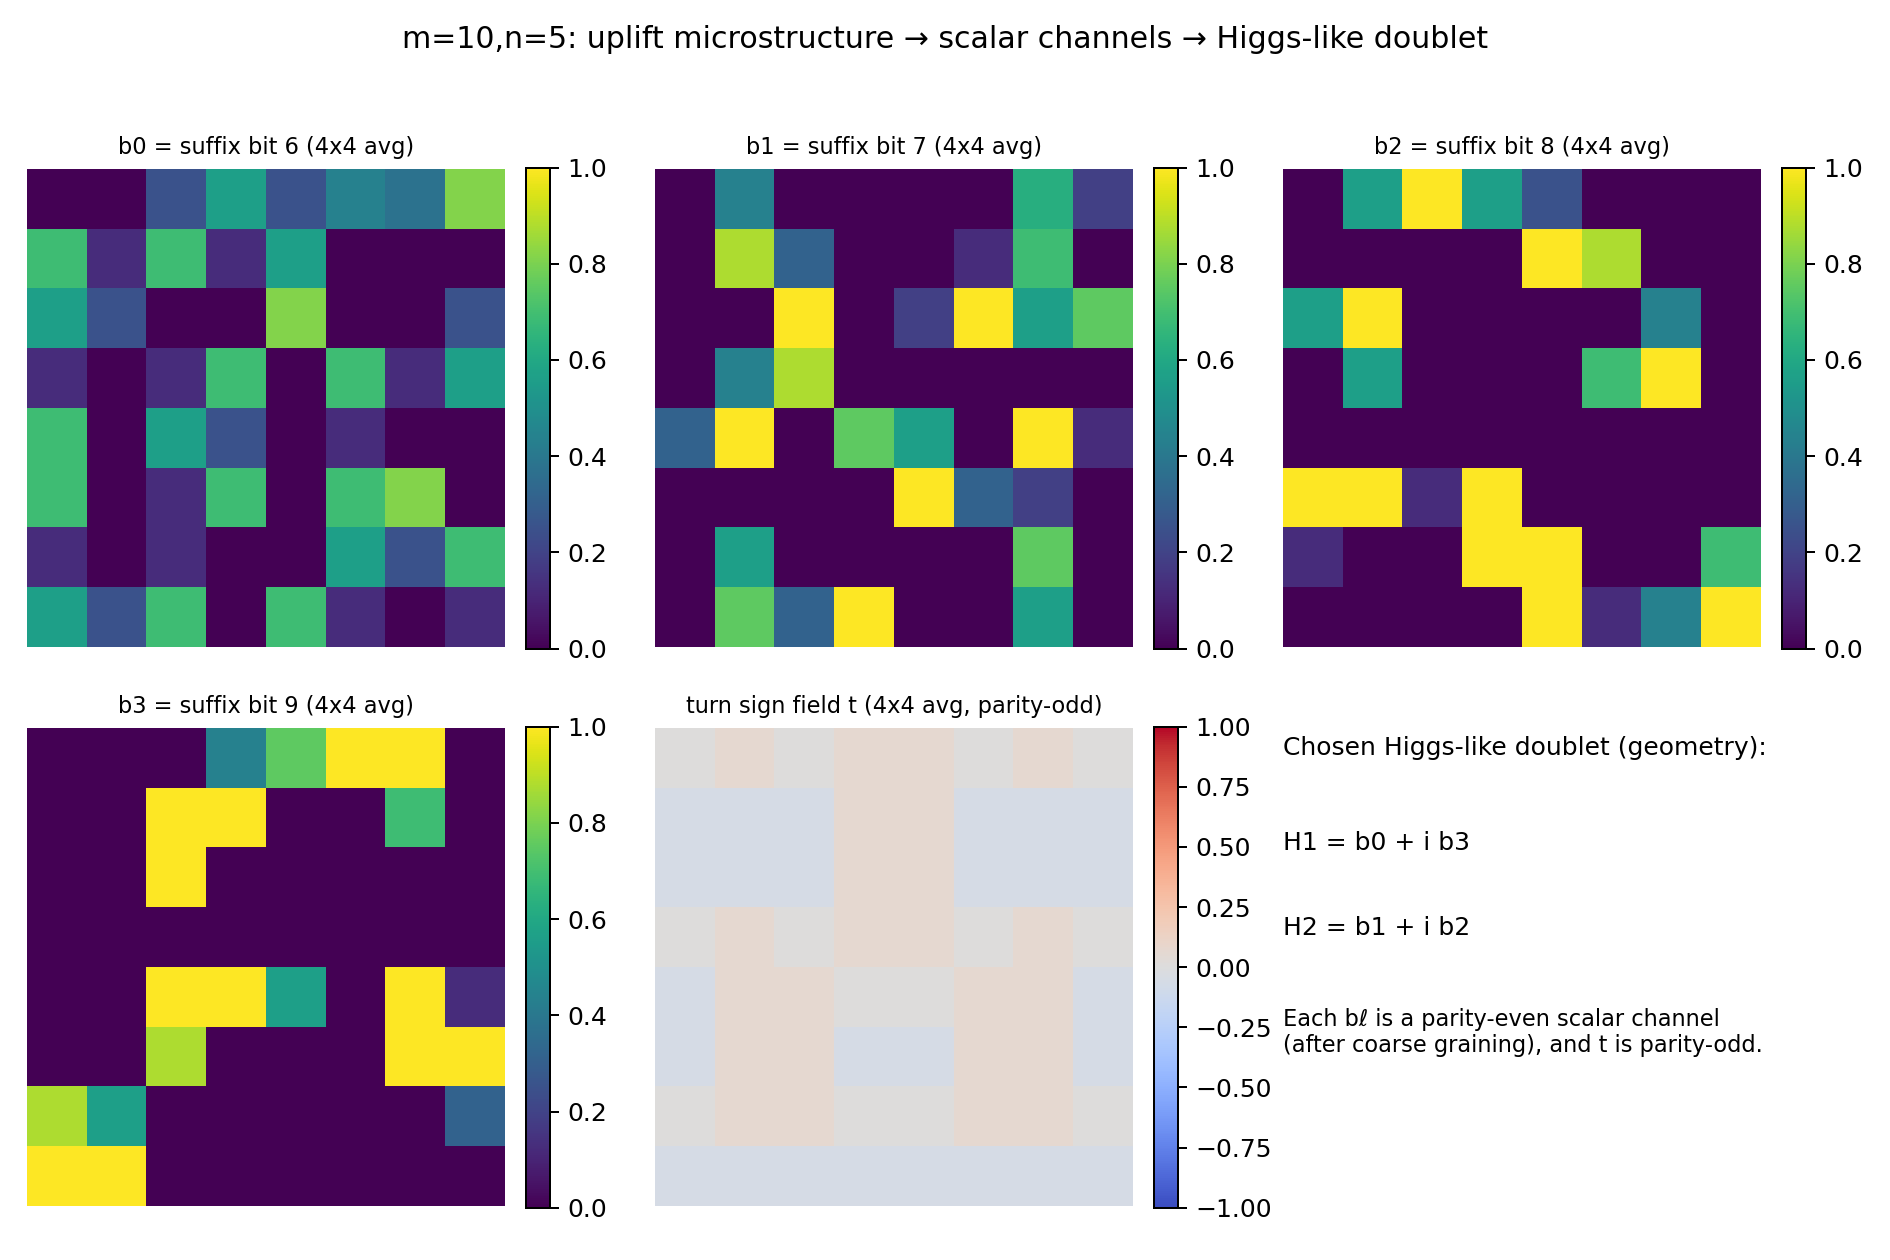
\includegraphics[width=\textwidth]{figures/adaptive/higgs_geometry/higgs_doublet_structure_m10}
\caption{A Higgs-like scalar doublet from uplift microtexture on the balanced $2$D Hilbert screen at $(m,n)=(10,5)$ (interface). Each panel shows one coarse-grained suffix-bit channel $\overline b_j$ (a parity-even scalar observable by construction), contrasted with the parity-odd turn-sign field of the Hilbert traversal. The deterministic bundling $H_1=\overline b_0+\iu\,\overline b_3$ and $H_2=\overline b_1+\iu\,\overline b_2$ provides a concrete protocol-level representative of a scalar doublet supported by uplift texture.}
\label{fig:higgs_doublet_structure_m10_2d}
\end{figure}

\begin{figure}[t]
\centering
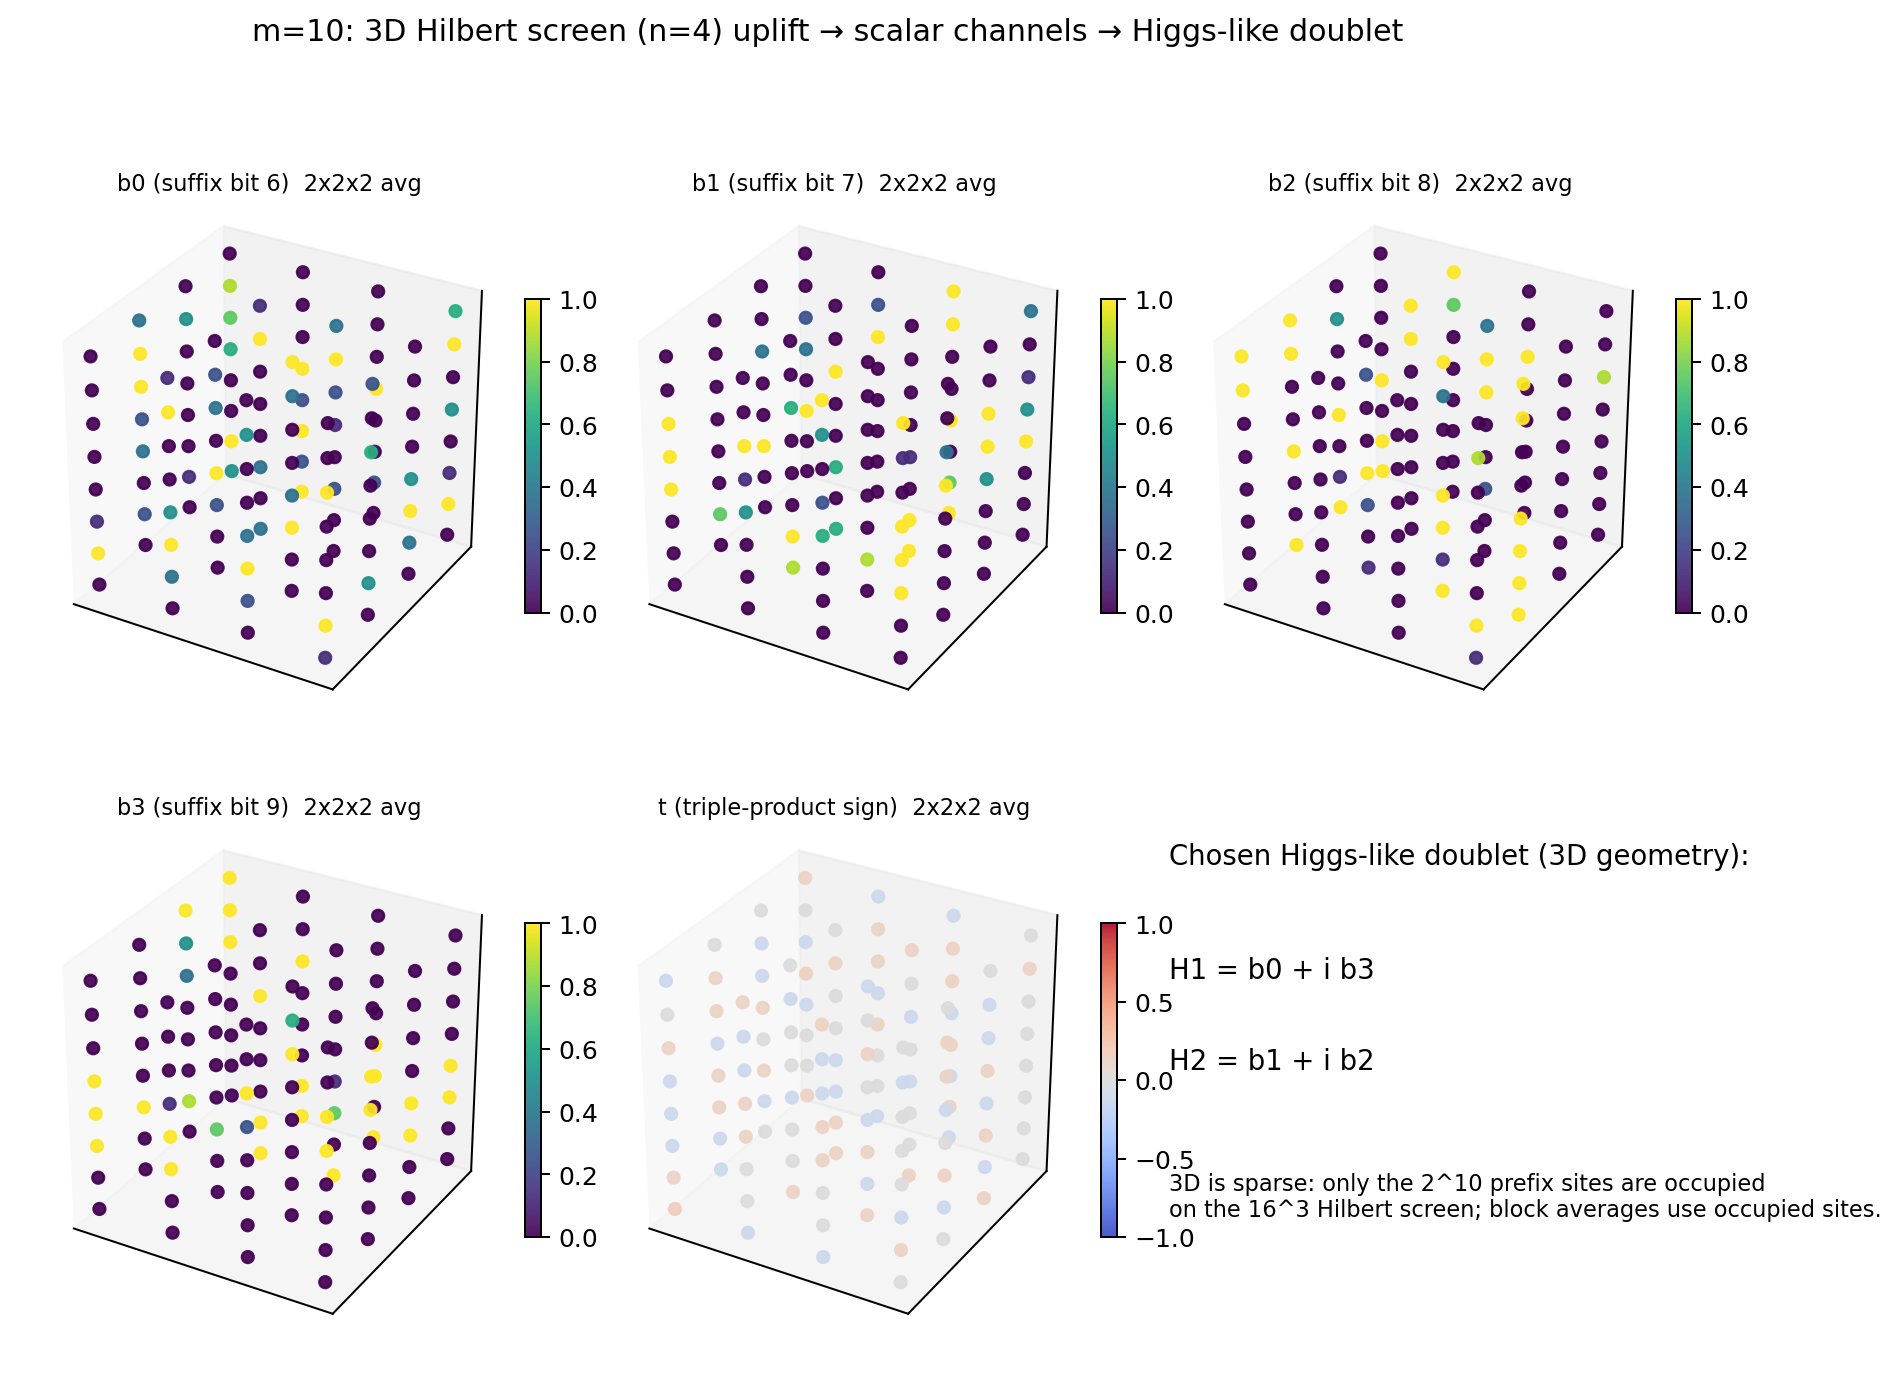
\includegraphics[width=\textwidth]{figures/adaptive/higgs_geometry/higgs_doublet_structure_m10_3d}
\caption{The same uplift-derived scalar-doublet construction displayed on a $3$D Hilbert screen (interface). Here $(m,n_3)=(10,4)$ embeds the first $2^{10}$ scan indices as a prefix of the finite $3$D Hilbert traversal on the $16^3$ cube (sparse occupancy); the scalar channels are coarse-grained by $2\times 2\times 2$ block averages on occupied blocks. The resulting canonical bundling agrees with the $2$D instance in Figure~\ref{fig:higgs_doublet_structure_m10_2d}.}
\label{fig:higgs_doublet_structure_m10_3d}
\end{figure}

\begin{remark}[Coupling scalars to connections (interface viewpoint)]
In lattice gauge theory, gauge fields live on links while scalar fields can be modeled as site variables transforming in a representation of the gauge group, with gauge-covariant nearest-neighbor couplings that reduce to $(D_\mu H)^\dagger(D^\mu H)$ in a continuum limit \cite{Wilson1974,KogutSusskind1975HamiltonianLGT,Rothe2012}.
In the present protocol language, this provides a concrete modeling route for scalar-sector closure (Proposition~\ref{prop:scalar_sector_closed}): allow the local implementation cost of compensating transport to depend on a coarse-grained scalar observable (Definition~\ref{def:coarse_grained_scalar}), yielding a site-dependent modulation of transport/holonomy statistics without introducing a new minimal stable type at $m=6$.
\end{remark}

\subsection{Protocol flow under uplift and coarse graining (interface)}
\label{subsec:protocol_flow_interface}

The program treats finite resolution as primary: both the window length $m$ and the spatial addressing scale $n$ are protocol parameters.
Changing resolution (uplift in $m$ and/or $n$) and applying coarse graining are therefore the protocol-native candidates for a discrete renormalization step.
In this paper, the protocol flow law is fixed explicitly as a discrete uplift--coarse-graining flow together with a standard RG dictionary in the resolution coordinate $r$ \cite{Wilson1974,Rothe2012}.


\begin{definition}[Protocol flow step and flowing objects]\label{def:protocol_flow_step}
Fix a family of protocol parameters $(m,n)$ and a chosen coarse-graining map $\mathsf{C}$ on the Hilbert-addressed grid (e.g.\ block averaging or kernel readout).
The \emph{protocol flow step} is the deterministic update
\[
(m,n)\mapsto(m',n')
\]
together with the induced map on observables obtained by:
(i) recomputing the finite stable sector $X_{m'}$ and intrinsic invariants at the new window length,
(ii) pushing observables forward/backward along the canonical prefix projection(s) $\pi_{m'\to m}$ (Appendix~\ref{app:functorial_refinement}),
and (iii) applying $\mathsf{C}$ to obtain coarse observables.
The \emph{flowing objects} are any protocol observables defined at finite resolution (stable-type counts, degeneracy histograms, holonomy distributions, bounded-complexity minimizers, and derived effective couplings defined as functions of these invariants).
\end{definition}

\begin{proposition}[RG dictionary in the Fibonacci resolution coordinate]\label{prop:rg_dictionary_r}
Let $\mu(r)=\mu_0\,\varphi^{\,r}$ be the Fibonacci resolution map (Section~\ref{subsec:mass_resolution_coordinate}) and let $g(\mu)$ be any scale-dependent effective parameter with a standard RG equation $\dd g/\dd\log\mu=\beta(g)$ away from thresholds.
Then, in the resolution coordinate,
\[
\frac{\dd g}{\dd r}=(\log\varphi)\,\beta(g).
\]
\end{proposition}
\begin{proof}
Since $\log\mu=\log\mu_0+r\log\varphi$, one has $\dd/\dd r=(\log\varphi)\,\dd/\dd\log\mu$.
\end{proof}


